\documentclass[main.tex]{subfiles}

\begin{document}

\section{A1 Git: Repository erzeugen}

\renewcommand{\labelenumi}{\arabic{enumi}.}
\begin{enumerate}
\item  Lassen Sie sich die installierte Version von Git ausgeben.
\item  Konfigurieren Sie in Git Ihren Benutzernamen und Ihre E-Mail-Adresse. Überprüfen Sie, ob die Konfiguration richtig ist.
\item  Erzeugen Sie auf einem Git-Server Ihrer Wahl, zum Beispiel auf dem GitLab-Server der FH Aachen, ein leeres Remote-Repository.
\item  Klonen Sie das neue Repository in ein neues Arbeitsverzeichnis auf Ihrem Rechner.
\item  Erstellen Sie in dem neuen Arbeitsverzeichnis eine Hello-World-Anwendung in der Programmiersprache Ihrer Wahl, z.B. Java, C\# oder Python (die Sprache sollte allerdings auf Textdateien mit Quellcode basieren).
\item  Lassen Sie sich den aktuellen Status ausgeben und übertragen Sie die Änderungen in Ihr lokales Repository.
\item  Bringen Sie das Remote-Repository auf den neuesten Stand.
\item  Ergänzen Sie in Ihrem Quellcode einige Inline-Kommentare, z.B. Autor und Datum.
\item  Übertragen Sie alle Änderungen in das Remote-Repository.
\item  Ergänzen Sie eine geeignete .gitignore-Datei für Ihr Projekt, um keine generierten Dateien in die Repositories zu übertragen. Löschen Sie ggf. alle Dateien im lokalen und im Remote-Repositories, die dort nicht hingehören.
\item  Benennen Sie mindestens eine Datei lokal um und stellen Sie sicher, dass die Umbenennung auch im Remote-Repository erfolgreich war.
\item  Führen Sie eine Änderung am Quellcode durch und machen Sie die Änderung wieder rückgängig, indem Sie den letzten Stand des lokalen Repository wiederherstellen.
\end{enumerate}

\subsection{Lösung 1}

\begin{figure}[H]
    \makebox[\textwidth][c]{
        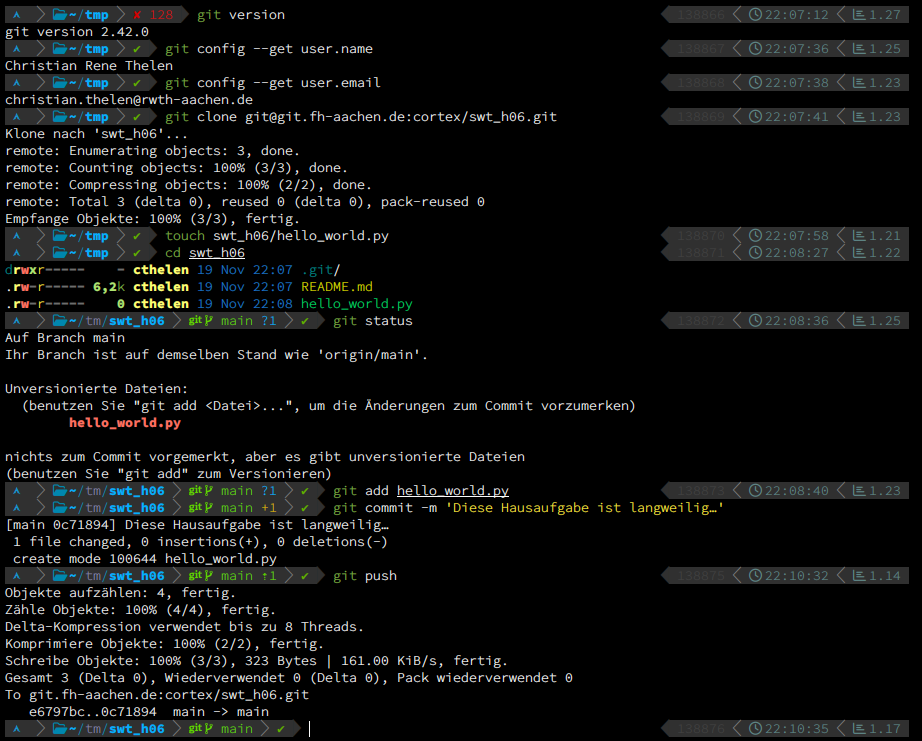
\includegraphics[width=1.2\linewidth]{s1.png}
    }
    \caption{Aufgabe 1, Nr. 1-7}
    \label{fig:a1}
\end{figure}

\begin{figure}[H]
    \makebox[\textwidth][c]{
        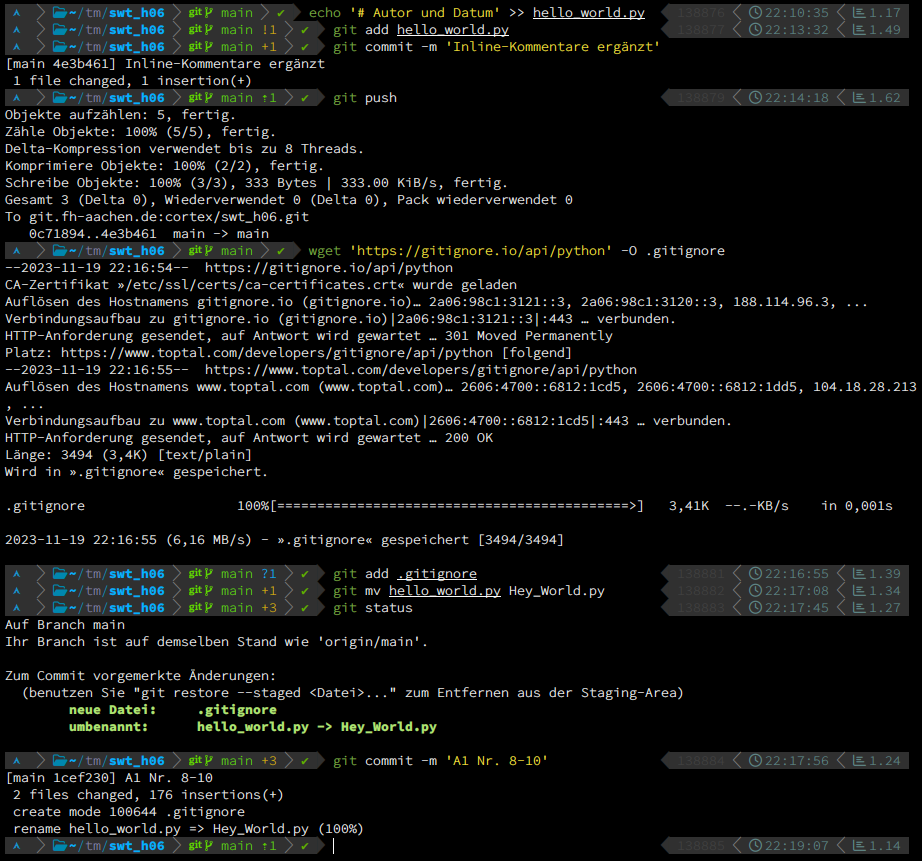
\includegraphics[width=1.2\linewidth]{s2.png}
    }
    \caption{Aufgabe 1, Nr. 8-11}
    \label{fig:a1}
\end{figure}

\begin{figure}[H]
    \makebox[\textwidth][c]{
        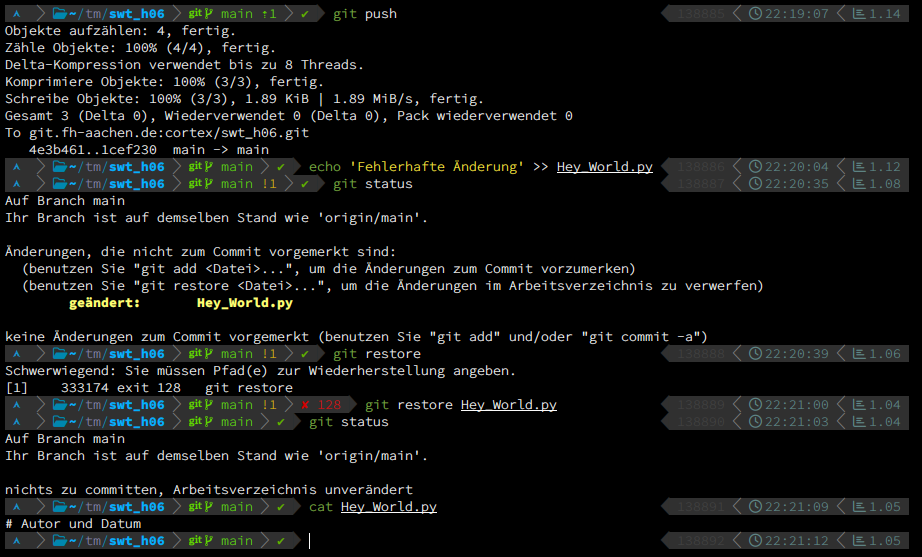
\includegraphics[width=1.2\linewidth]{s3.png}
    }
    \caption{Aufgabe 1, Nr. 12}
    \label{fig:a1}
\end{figure}

\end{document}
